\documentclass[a4paper]{article}
\usepackage[utf8]{inputenc}
\usepackage[T1]{fontenc}
\usepackage{textcomp}
\usepackage{amsmath, amssymb, amsthm}
\usepackage{geometry}
\usepackage{tikz-cd}
\usepackage{mdframed}
\usepackage{microtype}
\usepackage{hyperref}
\usepackage{cleveref}

\usepackage[backend = biber, style = alphabetic]{biblatex}
\addbibresource{../references.bib}

% figure support
\usepackage{import}
\usepackage{xifthen}
\usepackage[textsize=tiny,colorinlistoftodos,obeyDraft]{todonotes}
\newcommand{\question}[1]{\todo[color=green!40]{#1}}
\usepackage{pdfpages}
\usepackage{transparent}
\newcommand{\incfig}[1]{%
	\def\svgwidth{\columnwidth}
	\import{./figures/}{#1.pdf_tex}
}

\pdfsuppresswarningpagegroup=1


\newcommand{\N}{\mathbb{N}}
\newcommand{\Z}{\mathbb{Z}}
\newcommand{\Q}{\mathbb{Q}}
\newcommand{\C}{\mathbb{C}}
\newcommand{\R}{\mathbb{R}}
\newcommand{\F}{\mathbb{F}}
\newcommand{\pro}{\mathbb{P}}
\newcommand{\aff}{\mathbb{A}}
\newcommand{\ltr}{\par \noindent \framebox[1\width]{ $\implies$ } \hspace{.2cm}}
\newcommand{\rtl}{\par \noindent \framebox[1\width]{ $\impliedby$ } \hspace{.2cm} }

\DeclareMathOperator{\coker}{coker}
\DeclareMathOperator{\id}{Id}
\DeclareMathOperator{\im}{Im}
\DeclareMathOperator{\spec}{Spec}
\DeclareMathOperator{\maxspec}{MaxSpec}
\DeclareMathOperator{\spf}{Spf}
\DeclareMathOperator{\proj}{Proj}
\DeclareMathOperator{\red}{red}
\DeclareMathOperator{\trop}{trop}
\DeclareMathOperator{\trdeg}{TrDeg}
\DeclareMathOperator{\divisor}{Div}
\DeclareMathOperator{\cov}{Cov}

\newcommand{\into}{\hookrightarrow}
\newcommand{\onto}{\twoheadrightarrow}
\newcommand{\divides}{\mid}
\newcommand{\notdivides}{\nmid}
\newcommand{\Gan}{\ensuremath{\mathbb{G} _m ^{\mathrm{an}}}}
\newcommand{\an}{{}^{\text{an}}}
\newcommand{\cox}{\widehat{\otimes}}

\newcommand{\st}{%
  \nonscript\;
  \ifnum\currentgrouptype=16
    \,\middle|\,
  \else
    \,|\,
  \fi
  \nonscript\;}

\theoremstyle{definition}
\newtheorem{definition}{Definition}[subsection]
\newtheorem{remark}[definition]{Remark}
\newtheorem{theorem}[definition]{Theorem}
\newtheorem{example}[definition]{Example}
\newtheorem{lemma}[definition]{Lemma}
\newtheorem{claim}[definition]{Claim}
\newtheorem{proposition}[definition]{Proposition}
\newtheorem{exercise}[definition]{Exercise}
\newtheorem{corollary}[definition]{Corollary}


\author{Micha\"el Maex}


\title{Weight Functions}
\author{Michaël Maex}
\begin{document}

\maketitle

\tableofcontents



\todototoc
\listoftodos
\pagebreak

%The main paper I aim to understand in this document is \cite{bakerWeightFunctionsBerkovich2016}. 
%For this we will often need to look at \cite{nicaiseBerkovichSkeletaBirational2016} and sometimes at \cite{mustataWeightFunctionsNonArchimedean2015}. 

We might ask ourselves what a good notion for a minimal skeleton might be. 
A wish list of good properties for such a skeleton $\sk(X)$ is the following. 
\begin{itemize}
	\item The minimal skeleton needs to capture all information about the ``shape'' of $X\an$. 
		This means that the inclusion $\sk(X) \into X\an$ is a homotopy equivalence and it has to contain all all divisorial points whose associated minimal component is not rational.
	\item $\sk(X)$ is canonical. 
	\item $\sk(X)$ is well behaved under (nice) base change. 
\end{itemize}
For a curve $C$ of positive genus there is a canonical minimal skeleton $\sk(\mathscr C_\text{min} )$, with $\mathscr C_\text{min} $ the minimal snc-model.
However, this does not generalize to higher dimensions as not every variety has a minimal snc-model. 
Another drawback is that $\sk(\mathscr C_\text{min})$ is not functorial under base change. 

In \cite{mustataWeightFunctionsNonArchimedean2015} M.\ Mustaţă and J.\ Nicaise construct what they call the \emph{essential skeleton}.
It is defined for any variety with a semi-ample canonical line bundle, which is a much larger class of varieties than those with minimal snc-models. 
In particular, this includes every curve of non-zero genus. 
The essential skeleton is canonical, contains the shape of $X\an$ in the sense of the first wish and it pulls back under tame base-change. 
As we will see at the end of this section is even has some nice properties under some finite morphisms between curves. 
The main tool in defining it are weight functions. 

\subsection{Weight functions} \label{sec:weight_functions}
Given a variety $X$, a weight function is a piecewise $\Z$-affine linear function corresponding to a rational section $\sigma$ of the canonical line bundle. 
They are an important tool to study skeleta because if $\sigma$ is a regular section then the associated weight function $\wt_\sigma$ is strictly increasing away from every skeleton associated to a snc-model. 
So the minimal locus $\minloc \wt_\sigma$ has to be contained in every skeleton of $X$. 
This gives us a way of identifying pieces of a skeleton. 
Taking all these pieces together is the essential skeleton. 
We will only work in the context of curves. 
\nomenclature[minloc]{$\minloc f$}{The minimal locus of the function $f$}

\begin{definition}\label{def:log_cannonical_bundle}
	Let  $\mathscr C$ be a normal proper model of a curve $C $. 
	We define the \emph{log-canonical bundle of $\mathscr C$} to be \[
		\omega_{\mathscr C}^{\text{log}}  = \omega_{\mathscr C / R}(\mathscr C_{s, \text{red}} - \mathscr C_s)
	,\] 
	where $\omega_{\mathscr C}$ is the canonical bundle of $\mathscr C$ and $\mathscr C_{s, \text{red}}$ is the divisor on $\mathscr C$ that contains every irreducible component of $\mathscr C_s$ with multiplicity $1$.  
\end{definition}
\nomenclature[log]{$\omega^{\text{log}}_{\mathscr C}$}{The log-canonical bundle on $\mathscr C$}

Note that the restriction of $\omega_{\mathscr C}^{\text{log}}$ to the generic fiber is the canonical bundle on $C$. 

\begin{remark}
	The log-canonical bundle is actually the analogue of the canonical bundle for log schemes. 
	In this case the $\mathscr C$ has a log structure induced by the special fiber. 
	But for our purposes we can work with the explicit definition above. 
\end{remark}
\begin{definition}
	Let $C $ be a curve.
	The \emph{$m$-pluricanonical line bundle} is the $n$-th tensor power of the ordinary canonical line bundle, $\omega_{C / K}^{\otimes m }$. 
	A \emph{$m$-pluricanonical form}  is a non-zero global section of $\omega_{C / K}^{\otimes m }$. 
	A \emph{$m$-pluricanonical section} is a non-zero rational section of $\omega_{C / K}^{\otimes m }$.
\end{definition}
\nomenclature[mp]{$\omega_{C / K}^{\otimes m }$}{The $m$-pluricanonical linebundle on $C$}
\begin{notation}
	Let $D$ be a Cartier divisor on a scheme $X$, and let $F$ be a prime divisor on $D$. 
	Then we write $\mult_{F}(D)$ for the coefficient of $F$ in $D$. 
\end{notation}

We first define the weight function on a divisorial point and then use a sort of expansion by continuity to define it on the whole of $C\an$. 
\begin{definition}\label{def:weight_function_divisorial_point}
	Let $C$ and $\sigma$ be rational section of $\omega_{C / K}^{\otimes m}$.
	Let $x$ be a divisorial point in $C\an$ and $\mathscr C$ be a regular model  with a irreducible component $F$ of multiplicity $N$ corresponding to $x$. 
	Let $\sigma'$ be the unique extension of $\sigma$ to a $m$-pluricanonical section. 
	Then we define the \emph{weight of $\sigma$ at $x$} to be \[
		\wt_\sigma(x) = \frac{\mult_F(\divisor(\sigma'))}{N}
	.\] 
\end{definition}
\nomenclature[wt]{$\wt_{\sigma}$}{The weight function of the pluricanonical section $\sigma$ on $X$}

\begin{remark}
	If one does not like to work with the log-canonical bundle, we can use an alternative definition that puts a minor error term in the definition of the weight. 
	Let $\sigma"$ be the extension of $\sigma$ to $\omega_{\mathscr C / R}^{\otimes m}$. Then \[
		\wt_{\sigma} = \frac{\mult_F(\divisor (\sigma")) + m}{N} - m
	.\] 
\end{remark}
One can prove that this definition is independent of the model $\mathscr C$ chosen. 
We extend the weight function to $\mathbb{H}(C)$ as follows.
\begin{definition}\label{def:weight_function}
	Let $C$ be a curve and $\sigma$ a rational section of $\omega_{C / K}^{\otimes m}$. 
	Then we define the \emph{weight function} $\wt_{\sigma}: \mathbb{H}(C) \to \R$ to be the unique function such that 
	\begin{itemize}
		\item The restriction $\wt_{\sigma}|_{\sk(\mathscr C)}$ is continuous with respect to the metric topology on $\sk(\mathscr C)$ for any snc-model $\mathscr C$, 
		\item on divisorial points $x$ the value of $\wt_{\sigma}(x)$ agrees with \cref{def:weight_function_divisorial_point}.
	\end{itemize}
\end{definition}

The weight function can even be extended to the entirety of $C\an$, but then it may take $\pm \infty$ as values on the type 1 points. See \cite[§4.5.4]{mustataWeightFunctionsNonArchimedean2015}


Various tools and techniques for computing weight functions on curves can be found in \cite{bakerWeightFunctionsBerkovich2016}. 
These will be useful in \cref{chap:a_berkovich_approach_to_classifying_elliptic_curves}. 

\subsection{The essential skeleton $\sk(C)$}\label{sec:the_essential_skeleton_sk_c$}

Weight functions are interesting for studying models because when $\sigma$ is a $m$-pluricanonical form, i.e.\ a non-zero global section, then $\wt_\sigma$ is strictly increasing away from any skeleton associated to a snc-model. 
This is made precise in the following theorem. 
\begin{proposition}\label{prop:weight_function_increase}
	Let $\mathscr C$ be a snc-model of a curve $C$ and $\sigma$ be $m$-pluricanonical form on $C$ (i.e.\ a global section).
	Let $\rho_{\mathscr C}: C\an \to \sk(\mathscr C)$ be the retract from \cref{prop:retract_analytification_skeleton}. 
	Let $x \in C\an $ be any point. 
	Then \[
		\wt_\sigma(x) \ge \wt_\sigma(\rho_{\mathscr C}(x))
	,\] 
	with equality if and only if $x \in \sk(\mathscr C)$. 
\end{proposition}
\begin{proof}
	See \cite[prop.\ 4.4.4]{mustataWeightFunctionsNonArchimedean2015}. 
\end{proof}

\begin{definition}[Kontsevich–Soibelman skeleton]\label{def:KS_skeleton}
	Let $\mathscr C $ be curve and $\sigma$ a rational pluricanonical form. 
	Then we define the \emph{Kontsevich-Soibelman skeleton of $\sigma$} to be \[
		\sk(C, \sigma) = \minloc \wt_{\sigma}
	.\]  
	Here $\minloc f$ (the minimal locus) is the set where the function $f$ attains its infimum.
\end{definition}
\nomenclature[skcw]{$\sk(C, \sigma)$}{The Kontsevich-Soibelman skeleton on $C$ of $\sigma$}
\begin{lemma}
	Let $\sigma$ be a $m$-pluricanonical form and $\mathscr C$ a snc-model of $C$. 
	Then $\sk(C, \sigma) \subset  \sk(\mathscr C)$
\end{lemma}
\begin{proof}
	This follows from \cref{prop:weight_function_increase}, and the definition of the Kontsevich-Soibelman skeleton. 
\end{proof}
Calling the Kontsevich-Soibelman skeleton a skeleton might be slightly misleading as it might not have the same homotopy type as $C\an$. 
Note that for general $\sigma$ it might even be that $\sk(C, \sigma)$ is empty. 
But if $\sigma$ is a form then $\sk(C, \sigma)$ may be computed on $\sk (\mathscr C)$ for any snc-model $C$ by \cref{prop:weight_function_increase}. 
As $\sk(\mathscr C)$ is compact we know that $\wt_{\sigma}$ attains its minimum on $\sk(\mathscr C)$ and thus $\sk(C, \sigma)$ is non-empty. 
In fact $\sk(C, \sigma)$ will always be the union of edges in $\sk(\mathscr C)$. 
Still $\sk(C, \sigma)$ might only be a small part $\sk(\mathscr C)$. 

The solution to this is to take the union of many Kontsevich-Soibelman skeleta.
\begin{definition}[essential skeleton]
	Let $C$ be a curve. 
	Then the \emph{essential skeleton of $C$} is \[
		\sk(C) = \bigcup_{\sigma} \sk(C, \sigma)
	\] 
	where $\sigma$ runs over all $m$-pluricanonical forms of $C$ for all $m > 1$. 
\end{definition}
\nomenclature[sk]{$\sk(C)$}{The essential skeleton of $C$}
\begin{remark}\label{rem:sufficiently_divisible_pluriconanonical}
	Note that in the definition of the essential skeleton, it is sufficient to let $\sigma$ range over all $m$-pluricanonical forms with $m$ sufficiently divisible. 
	This is because if $\sigma$ is a $m$-pluricanonical form, then $\sigma^{\otimes d}$ is a $md$-pluricanonical form and $\wt_{\sigma{\otimes d}} = d\cdot \wt_{\sigma}$. 
	So $\sk(C, \sigma) = \sk(C, \sigma^{\otimes d})$. 
\end{remark}
\begin{remark}
	While weight functions are defined for \emph{rational sections} of the pluricanonical line bundle $\omega_{C / K}^{\otimes m}$, when we define the essential skeleton we consider the weight functions where $\sigma$ is a \emph{form}, i.e.\ a global section of $\omega_{C / K} ^{\otimes m}$. 
	So it is important to make the distinction between \emph{rational sections} and \emph{forms}.
\end{remark}

It is not at all clear from the definition that the essential skeleton actually captures the shape of $C\an$, i.e.\ has the same homotopy type and contains all the points of non-zero genus. 
If $C = \pro^{1}_K$ then $\sk(C)$ is empty because there are no pluricanonical sections. Indeed the $m$-th pluricanonical line bundle is isomorphic to  $\mathcal{O}(-2m)$, which does not have global sections. 
But for curves of non-zero genus the canonical line bundle is semi-ample and thus $\sk(C)$ is non-zero. 

If $C$ is a curve of genus $g(C) > 0$ then there is a way of obtaining $\sk(C)$ from $\sk(\mathscr C_\text{min} )$, where $\mathscr C _\text{min}$ is the minimal regular model and removing some superfluous tails or rational curves.  

\begin{definition}
	Let $\mathscr C$ be a snc-model for a curve $C$. 
	An irreducible component $F$ of $\mathscr C_s$ (vertex in $\Delta(\mathscr C)$) is called \emph{inessesential}, if in the dual graph it belongs to a path of vertices $v_1, \ldots, v_n$ of genus $0$ with the valency $v(v_1) = 1$, $v(v_{2}) = 2, \ldots, v(v_{n-1}) = 2, v(v_n) > 2$ and $F \ne v_n$. 
	Conversely a component/vertex if called \emph{essential} if it is not inessential. 
\end{definition}
See \cref{fig:inessential_components} for some examples of the essential and inessential vertices on a dual graph. 

\begin{figure}[h]
    \centering
    \incfig{inessential-components}
    \caption{Some hypothetical dual graphs with the inessential components colored red. 
    The numbers next to the vertices are the genus of that component if it differs form zero.}
    \label{fig:inessential_components}
\end{figure}

\begin{theorem}
	Let $C$ be a curve with genus $g(C) > 0$ and let $\mathscr C_\text{min} $ be the minimal snc-model of $C$. 
	Let $\Delta'$ be the complete subgraph of $\Delta(\mathscr C_\text{min} )$ with the essential vertices. 
	Then the essential skeleton is the image of $|\Delta'|$\[
		\sk(C) = \sk_{\mathscr C_\text{min} }(|\Delta'|)
	.\] 
\end{theorem}
\begin{proof}
	The proof is insightful as to obtain this result one needs to understand the relation between weight functions and the pluricanonical forms.
	Unfortunately it is too long to put in this thesis. 
	The interested reader is encouraged to look at \cite[thm 3.3.13]{bakerWeightFunctionsBerkovich2016}. 
\end{proof}
\begin{figure}[h]
	\centering
	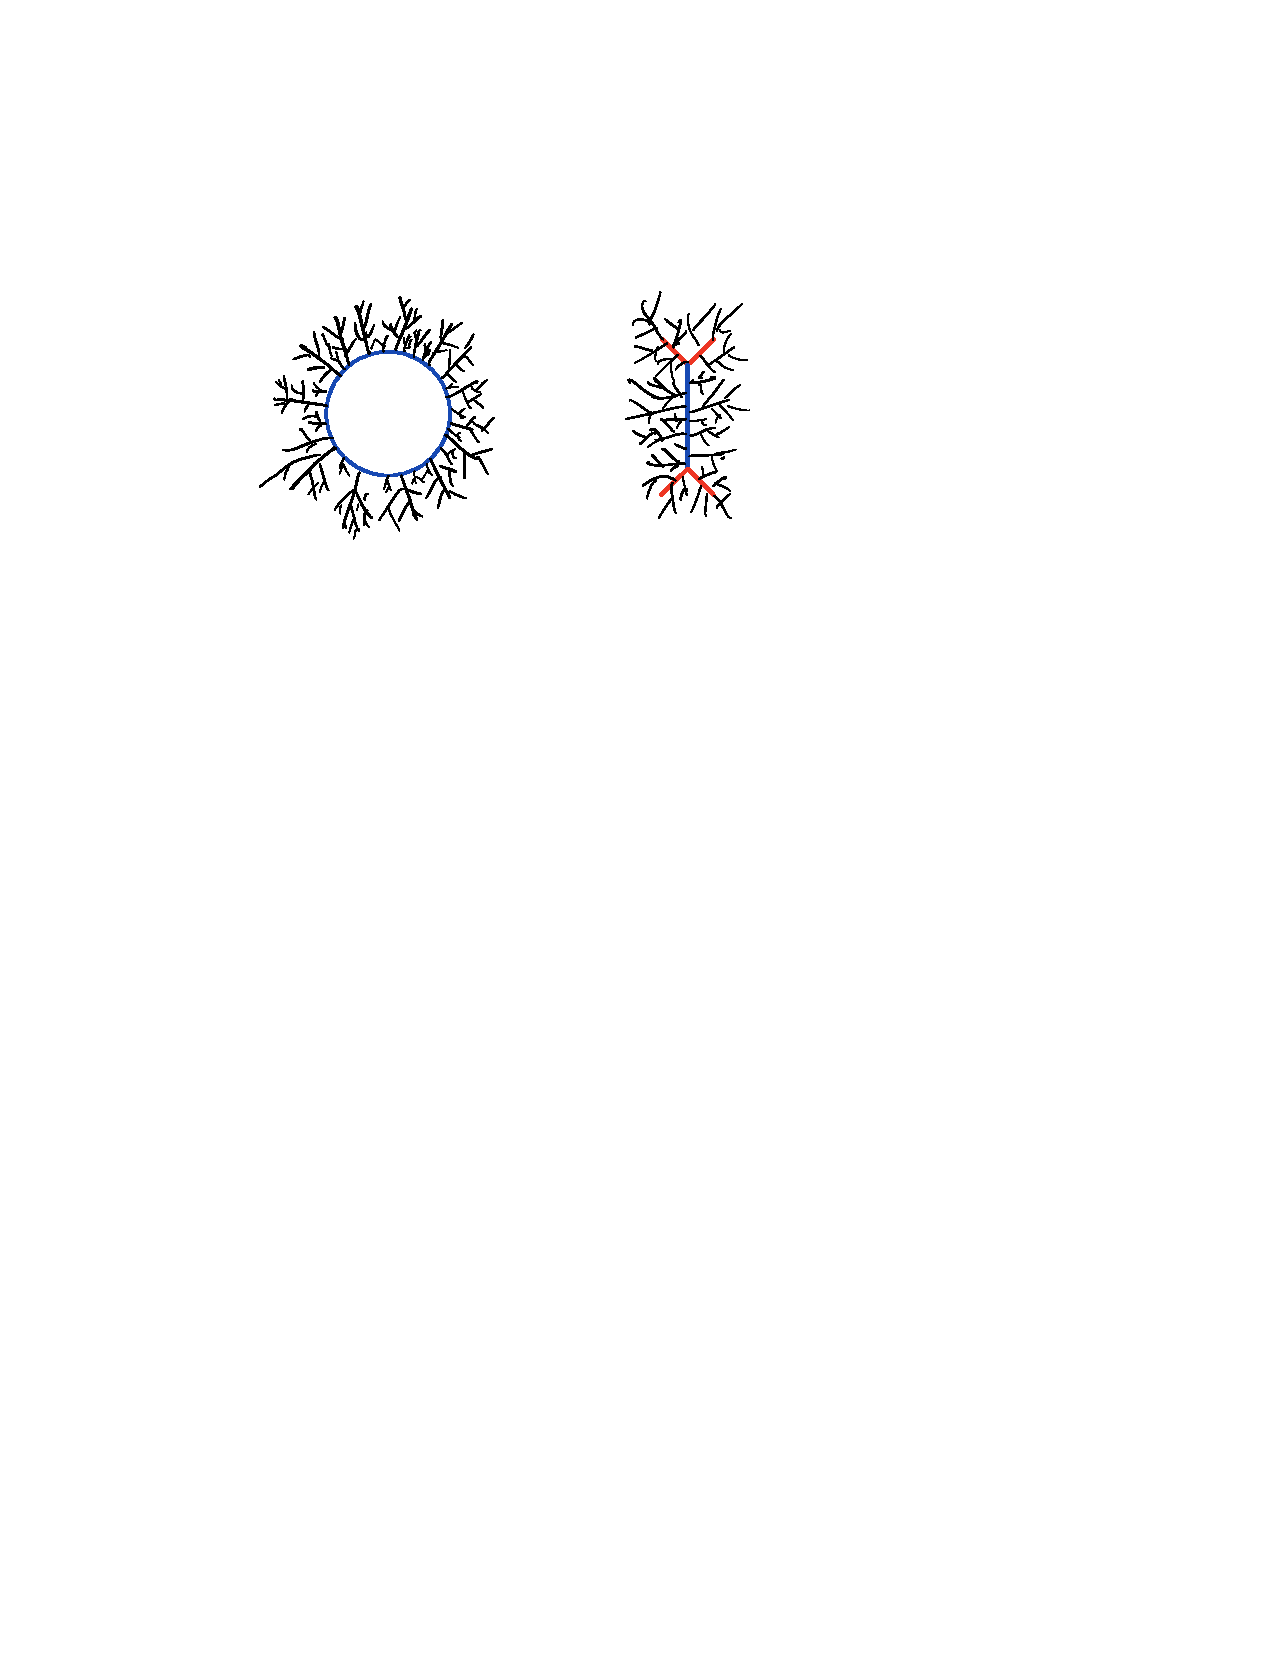
\includegraphics[width=0.6\textwidth]{chapters/weight/figures/essential_skeleton_elliptic.pdf}
	\caption{Artistic renderings of the analytification of an elliptic curve of type $\mathrm I_n, n \ge 1$ (left) and $\mathrm I_n^*, n \ge 1$ (right) with the essential skeleton in blue and the inessential bits of  $\sk(\mathscr E_\text{min} )$ in red. }
	\label{fig:}
\end{figure}


\section{Weight functions under morphisms of curves} \label{sec:weight_functions_under_morphisms_of_curves}

\begin{lemma}
	Let $\mathscr{E} \to \mathscr{P}$ be a morphism of morphism of models of $E$ and $P$ extending the map $f: E \to P$ such that the special fibres of $\mathscr E, \mathscr P$ consists one irreducible component $F, G$ with multiplicity $M, N$ respectively. 
	Suppose that the map $\psi: F \to G$ is purely inseparable of degree $f^{i}$.
	\[
	\begin{tikzcd}
		E \dar{f} \rar[hookrightarrow] & \mathscr E \dar{\phi} \rar[hookleftarrow] &  F \dar{\psi} \\
		P \rar[hookrightarrow] & \mathscr P \rar[hookleftarrow] &  G
	\end{tikzcd}
	.\] 
	Let $K_E = f^* K_P$ and $K_{\mathscr E}, K_{\mathscr P}$ be the extensions of $K_E, K_P$ in $\omega_\mathscr E, \omega_\mathscr P$ respectively. 
	Then \todo{Yeah, then what?}
\end{lemma}
\begin{proof}
	First note that $\mathscr{E} _s = \phi^* \mathscr{P} _s$. Hence 
	\begin{equation}\label{eq:lem_insep_ext_pulback_irred}
		\frac{M}{N} F = f^* G
	.\end{equation} 
	As the morphism $\psi$ purely inseparable of degree $f^{i}$ we have 
	\begin{equation}\label{eq:insep_ext_can_bundle}
		f^{i} K_F = \psi^* K_G
	.\end{equation}
	Also recall the adjunction formula 
	\begin{equation}\label{eq:adjunction_insep_ext}
		(K_\mathscr E + F)|_F = K_F, \quad (K_\mathscr P + G)|_ G = K_G 
	\end{equation}
	The ramification divisor $\ram_\phi$ is defined as \[
		\ram_\phi= \phi^* K_\mathscr P - K_\mathscr E
	.\] 
	By looking at the generic fibre we see that the horizontal component of $\ram _\phi$ is just $\overline{\ram_f}$. 
	The vertical component is $a\cdot F$ for some $a \in \Z$. 
	So 
	\begin{equation}
		\ram_\phi = \overline{\ram_f} + a \cdot F
	\end{equation}
	In order to compute $\ram_\phi$ we need to find $a$ and we do this by resticting to the reduced special fibres. 
	\begin{align*}
		0 &= (\ram_\phi + K_\mathscr E - \phi^* K_{\mathscr P})|_F\\
		  &= \overline{\ram_f}|_F + a\cdot F|_F + K_\mathscr E|_F - \psi^*(K_\mathscr P|_G) \\
		  &= \overline{\ram_f}|_F + (a-1) \cdot F|_F + K_F - \psi^*(K_G - G|_G) & \text{using \eqref{eq:adjunction_insep_ext}}\\
		  &= \overline{\ram _f}|_F + (a - 1)\cdot F|_F + (1-f^{i})\cdot K_F + (\phi^* G)|_F & \text{using \eqref{eq:insep_ext_can_bundle}} \\
		  &= \overline{\ram_f}|_F + \left(a-1 + \frac{M}{N}\right) \cdot F|_F + (1 - f^{i}) \cdot K_F  & \text{using \eqref{eq:lem_insep_ext_pulback_irred}}
	.\end{align*}
	To find $a$ we can look at the degrees. 
	So we get 
	\begin{align*}
		0 &= \left( \overline{\ram_f}, F \right) + \left(a - 1 + \frac{M}{N}\right) \left(F, F\right) + (1-f^{i}) (2g_F -2) \\
		\iff a &= \frac{(\overline{\ram_f}, F) + (1-f^{i})(2g_F -2)  }{(F, F)} + 1 - \frac{M}{N}
	\end{align*}
	where $g_F$ is the genus of $F$ and $(\overline{\ram_f})$ can be intepreted as the number of ramification points that specialize to $F$. 


	Now lets see what this does to the weight functions at $F$. 
	We have 
	\begin{align*}
		\wt_{f^* K_P}(F) &= \frac{\mult_F K_{\mathscr E} + 1}{M} \\
		&= \frac{\mult_F f^*K_{\mathscr P} - \mult_F \ram_\phi + 1}{M} \\
		&= \frac{\frac{M}{N}\mult_G K_{\mathscr P} - a + 1}{M} \\
		&= \frac{\mult_G K_{\mathscr P} + 1}{N} - \frac{a - 1 + M / N}{M} \\
		&= \wt_{K_P}(G) - \frac{(\overline{\ram_f}, F) + (1 - f^{i})(2g_F - 2)}{(F, F)\cdot M} 
	.\end{align*}
\end{proof}
	\todo{I don't think the ramification divisor should end up on the final formula}
\begin{definition}
	Let $f: X \to Y$ be a map of smooth projective curves and $\omega$ be a pluricanonical form. 
	We define the \emph{weight difference} of $f, \omega$ for $\omega$ a rational section of $Y$ to be \[
		\wt_{\omega} \circ f\an - \wt_{f^* \omega} 
	.\] 
\end{definition}
\begin{remark}
	The weight function is indepentent of  $\omega$???? \todo{I think this is true?}
\end{remark}

\begin{corollary}
	Let $f: X \to Y$ be a galois cover of degree $d$ between projective smooth connected curves over $K$, such that $\ch K \nmid d$.  
	Then the weight difference is of $f$ is zero, hence \[
	\wt_{f^* \omega} = \wt_{\omega} \circ f\an  
	.\] 
\end{corollary}






\pagebreak
\printbibliography
\end{document}
